\documentclass[12pt]{article} 
% Formatting
\tolerance=1000
\usepackage[margin=1.2in]{geometry}


% Custom definitions
% To use this customization file, insert the line "% Custom definitions
% To use this customization file, insert the line "% Custom definitions
% To use this customization file, insert the line "\input{custom}" in the header of the tex file.

% Formatting

\tolerance=1000

% Packages

% \usepackage{amssymb,latexsym}
\usepackage{amssymb,amsfonts,amsmath,latexsym,amsthm}
\usepackage[usenames,dvipsnames]{color}
\usepackage[]{graphicx}
\usepackage[space]{grffile}
\usepackage{mathrsfs}   % fancy math font
% \usepackage[font=small,skip=0pt]{caption}
\usepackage[skip=0pt]{caption}
\usepackage{subcaption}
\usepackage{verbatim}
\usepackage{url}
\usepackage{bm}
\usepackage{dsfont}
\usepackage{extarrows}
\usepackage{multirow}
% \usepackage{wrapfig}
% \usepackage{epstopdf}
\usepackage{rotating}
\usepackage{tikz}
\usetikzlibrary{fit}					% fitting shapes to coordinates
%\usetikzlibrary{backgrounds}	% drawing the background after the foreground

% \usepackage[dvipdfm,colorlinks,citecolor=blue,linkcolor=blue,urlcolor=blue]{hyperref}
\usepackage[colorlinks,citecolor=blue,linkcolor=blue,urlcolor=blue]{hyperref}
%\usepackage{hyperref}
\usepackage[authoryear,round]{natbib}


%  Theorems, etc.

\theoremstyle{plain}
\newtheorem{theorem}{Theorem}[section]
\newtheorem{corollary}[theorem]{Corollary}
\newtheorem{lemma}[theorem]{Lemma}
\newtheorem{proposition}[theorem]{Proposition}
\newtheorem{condition}[theorem]{Condition}
% \newtheorem{conditions}[theorem]{Conditions}

\theoremstyle{definition}
\newtheorem{definition}[theorem]{Definition}
% \newtheorem*{unnumbered-definition}{Definition}
\newtheorem{example}[theorem]{Example}
\theoremstyle{remark}
\newtheorem*{remark}{Remark}
\numberwithin{equation}{section}


% footnote without number
\newcommand\blankfootnote[1]{%
  \begingroup
  \renewcommand\thefootnote{}\footnote{#1}%
  \addtocounter{footnote}{-1}%
  \endgroup
}
\makeatletter
\renewcommand\footnoterule{%
  \kern-3\p@
  \hrule\@width \textwidth
  \kern2.6\p@}
\makeatother

% Document-specific shortcuts
\newcommand{\btheta}{{\bm\theta}}
\newcommand{\bbtheta}{{\pmb{\bm\theta}}}

\newcommand{\commentary}[1]{\ifx\showcommentary\undefined\else \emph{#1}\fi}

\newcommand{\term}[1]{\textit{\textbf{#1}}}

% Math shortcuts

% Probability distributions
\DeclareMathOperator*{\Exp}{Exp}
\DeclareMathOperator*{\TExp}{TExp}
\DeclareMathOperator*{\Bernoulli}{Bernoulli}
\DeclareMathOperator*{\Beta}{Beta}
\DeclareMathOperator*{\Ga}{Gamma}
\DeclareMathOperator*{\TGamma}{TGamma}
\DeclareMathOperator*{\Poisson}{Poisson}
\DeclareMathOperator*{\Binomial}{Binomial}
\DeclareMathOperator*{\NormalGamma}{NormalGamma}
\DeclareMathOperator*{\InvGamma}{InvGamma}
\DeclareMathOperator*{\Cauchy}{Cauchy}
\DeclareMathOperator*{\Uniform}{Uniform}
\DeclareMathOperator*{\Gumbel}{Gumbel}
\DeclareMathOperator*{\Pareto}{Pareto}
\DeclareMathOperator*{\Mono}{Mono}
\DeclareMathOperator*{\Geometric}{Geometric}
\DeclareMathOperator*{\Wishart}{Wishart}

% Math operators
\DeclareMathOperator*{\argmin}{argmin}
\DeclareMathOperator*{\argmax}{argmax}
\DeclareMathOperator*{\Cov}{Cov}
\DeclareMathOperator*{\diag}{diag}
\DeclareMathOperator*{\median}{median}
\DeclareMathOperator*{\Vol}{Vol}
\newcommand{\logit}{\mathrm{logit}}

% Math characters
\newcommand{\R}{\mathbb{R}}
\newcommand{\Z}{\mathbb{Z}}
\newcommand{\E}{\mathbb{E}}
\renewcommand{\Pr}{\mathbb{P}}
\newcommand{\1}{\mathds{1}}
\newcommand{\V}{\mathbb{V}}

\newcommand{\A}{\mathcal{A}}
\newcommand{\C}{\mathcal{C}}
\newcommand{\D}{\mathcal{D}}
\newcommand{\Hcal}{\mathcal{H}}
\newcommand{\I}{\mathcal{I}}
\newcommand{\J}{\mathcal{J}}
\newcommand{\M}{\mathcal{M}}
\newcommand{\N}{\mathcal{N}}
\newcommand{\X}{\mathcal{X}}
\newcommand{\Zcal}{\mathcal{Z}}
\renewcommand{\P}{\mathcal{P}}

\newcommand{\T}{\mathtt{T}}
\renewcommand{\emptyset}{\varnothing}


% Miscellaneous commands
\newcommand{\iid}{\stackrel{\mathrm{iid}}{\sim}}
\newcommand{\matrixsmall}[1]{\bigl(\begin{smallmatrix}#1\end{smallmatrix} \bigr)}

\newcommand{\items}[1]{\begin{itemize} #1 \end{itemize}}

\newcommand{\todo}[1]{\emph{\textcolor{red}{(#1)}}}

\newcommand{\branch}[4]{
\left\{
	\begin{array}{ll}
		#1  & \mbox{if } #2 \\
		#3 & \mbox{if } #4
	\end{array}
\right.
}

% approximately proportional to
\def\app#1#2{%
  \mathrel{%
    \setbox0=\hbox{$#1\sim$}%
    \setbox2=\hbox{%
      \rlap{\hbox{$#1\propto$}}%
      \lower1.3\ht0\box0%
    }%
    \raise0.25\ht2\box2%
  }%
}
\def\approxprop{\mathpalette\app\relax}

% \newcommand{\approptoinn}[2]{\mathrel{\vcenter{
  % \offinterlineskip\halign{\hfil$##$\cr
    % #1\propto\cr\noalign{\kern2pt}#1\sim\cr\noalign{\kern-2pt}}}}}

% \newcommand{\approxpropto}{\mathpalette\approptoinn\relax}





" in the header of the tex file.

% Formatting

\tolerance=1000

% Packages

% \usepackage{amssymb,latexsym}
\usepackage{amssymb,amsfonts,amsmath,latexsym,amsthm}
\usepackage[usenames,dvipsnames]{color}
\usepackage[]{graphicx}
\usepackage[space]{grffile}
\usepackage{mathrsfs}   % fancy math font
% \usepackage[font=small,skip=0pt]{caption}
\usepackage[skip=0pt]{caption}
\usepackage{subcaption}
\usepackage{verbatim}
\usepackage{url}
\usepackage{bm}
\usepackage{dsfont}
\usepackage{extarrows}
\usepackage{multirow}
% \usepackage{wrapfig}
% \usepackage{epstopdf}
\usepackage{rotating}
\usepackage{tikz}
\usetikzlibrary{fit}					% fitting shapes to coordinates
%\usetikzlibrary{backgrounds}	% drawing the background after the foreground

% \usepackage[dvipdfm,colorlinks,citecolor=blue,linkcolor=blue,urlcolor=blue]{hyperref}
\usepackage[colorlinks,citecolor=blue,linkcolor=blue,urlcolor=blue]{hyperref}
%\usepackage{hyperref}
\usepackage[authoryear,round]{natbib}


%  Theorems, etc.

\theoremstyle{plain}
\newtheorem{theorem}{Theorem}[section]
\newtheorem{corollary}[theorem]{Corollary}
\newtheorem{lemma}[theorem]{Lemma}
\newtheorem{proposition}[theorem]{Proposition}
\newtheorem{condition}[theorem]{Condition}
% \newtheorem{conditions}[theorem]{Conditions}

\theoremstyle{definition}
\newtheorem{definition}[theorem]{Definition}
% \newtheorem*{unnumbered-definition}{Definition}
\newtheorem{example}[theorem]{Example}
\theoremstyle{remark}
\newtheorem*{remark}{Remark}
\numberwithin{equation}{section}


% footnote without number
\newcommand\blankfootnote[1]{%
  \begingroup
  \renewcommand\thefootnote{}\footnote{#1}%
  \addtocounter{footnote}{-1}%
  \endgroup
}
\makeatletter
\renewcommand\footnoterule{%
  \kern-3\p@
  \hrule\@width \textwidth
  \kern2.6\p@}
\makeatother

% Document-specific shortcuts
\newcommand{\btheta}{{\bm\theta}}
\newcommand{\bbtheta}{{\pmb{\bm\theta}}}

\newcommand{\commentary}[1]{\ifx\showcommentary\undefined\else \emph{#1}\fi}

\newcommand{\term}[1]{\textit{\textbf{#1}}}

% Math shortcuts

% Probability distributions
\DeclareMathOperator*{\Exp}{Exp}
\DeclareMathOperator*{\TExp}{TExp}
\DeclareMathOperator*{\Bernoulli}{Bernoulli}
\DeclareMathOperator*{\Beta}{Beta}
\DeclareMathOperator*{\Ga}{Gamma}
\DeclareMathOperator*{\TGamma}{TGamma}
\DeclareMathOperator*{\Poisson}{Poisson}
\DeclareMathOperator*{\Binomial}{Binomial}
\DeclareMathOperator*{\NormalGamma}{NormalGamma}
\DeclareMathOperator*{\InvGamma}{InvGamma}
\DeclareMathOperator*{\Cauchy}{Cauchy}
\DeclareMathOperator*{\Uniform}{Uniform}
\DeclareMathOperator*{\Gumbel}{Gumbel}
\DeclareMathOperator*{\Pareto}{Pareto}
\DeclareMathOperator*{\Mono}{Mono}
\DeclareMathOperator*{\Geometric}{Geometric}
\DeclareMathOperator*{\Wishart}{Wishart}

% Math operators
\DeclareMathOperator*{\argmin}{argmin}
\DeclareMathOperator*{\argmax}{argmax}
\DeclareMathOperator*{\Cov}{Cov}
\DeclareMathOperator*{\diag}{diag}
\DeclareMathOperator*{\median}{median}
\DeclareMathOperator*{\Vol}{Vol}
\newcommand{\logit}{\mathrm{logit}}

% Math characters
\newcommand{\R}{\mathbb{R}}
\newcommand{\Z}{\mathbb{Z}}
\newcommand{\E}{\mathbb{E}}
\renewcommand{\Pr}{\mathbb{P}}
\newcommand{\1}{\mathds{1}}
\newcommand{\V}{\mathbb{V}}

\newcommand{\A}{\mathcal{A}}
\newcommand{\C}{\mathcal{C}}
\newcommand{\D}{\mathcal{D}}
\newcommand{\Hcal}{\mathcal{H}}
\newcommand{\I}{\mathcal{I}}
\newcommand{\J}{\mathcal{J}}
\newcommand{\M}{\mathcal{M}}
\newcommand{\N}{\mathcal{N}}
\newcommand{\X}{\mathcal{X}}
\newcommand{\Zcal}{\mathcal{Z}}
\renewcommand{\P}{\mathcal{P}}

\newcommand{\T}{\mathtt{T}}
\renewcommand{\emptyset}{\varnothing}


% Miscellaneous commands
\newcommand{\iid}{\stackrel{\mathrm{iid}}{\sim}}
\newcommand{\matrixsmall}[1]{\bigl(\begin{smallmatrix}#1\end{smallmatrix} \bigr)}

\newcommand{\items}[1]{\begin{itemize} #1 \end{itemize}}

\newcommand{\todo}[1]{\emph{\textcolor{red}{(#1)}}}

\newcommand{\branch}[4]{
\left\{
	\begin{array}{ll}
		#1  & \mbox{if } #2 \\
		#3 & \mbox{if } #4
	\end{array}
\right.
}

% approximately proportional to
\def\app#1#2{%
  \mathrel{%
    \setbox0=\hbox{$#1\sim$}%
    \setbox2=\hbox{%
      \rlap{\hbox{$#1\propto$}}%
      \lower1.3\ht0\box0%
    }%
    \raise0.25\ht2\box2%
  }%
}
\def\approxprop{\mathpalette\app\relax}

% \newcommand{\approptoinn}[2]{\mathrel{\vcenter{
  % \offinterlineskip\halign{\hfil$##$\cr
    % #1\propto\cr\noalign{\kern2pt}#1\sim\cr\noalign{\kern-2pt}}}}}

% \newcommand{\approxpropto}{\mathpalette\approptoinn\relax}





" in the header of the tex file.

% Formatting

\tolerance=1000

% Packages

% \usepackage{amssymb,latexsym}
\usepackage{amssymb,amsfonts,amsmath,latexsym,amsthm}
\usepackage[usenames,dvipsnames]{color}
\usepackage[]{graphicx}
\usepackage[space]{grffile}
\usepackage{mathrsfs}   % fancy math font
% \usepackage[font=small,skip=0pt]{caption}
\usepackage[skip=0pt]{caption}
\usepackage{subcaption}
\usepackage{verbatim}
\usepackage{url}
\usepackage{bm}
\usepackage{dsfont}
\usepackage{extarrows}
\usepackage{multirow}
% \usepackage{wrapfig}
% \usepackage{epstopdf}
\usepackage{rotating}
\usepackage{tikz}
\usetikzlibrary{fit}					% fitting shapes to coordinates
%\usetikzlibrary{backgrounds}	% drawing the background after the foreground

% \usepackage[dvipdfm,colorlinks,citecolor=blue,linkcolor=blue,urlcolor=blue]{hyperref}
\usepackage[colorlinks,citecolor=blue,linkcolor=blue,urlcolor=blue]{hyperref}
%\usepackage{hyperref}
\usepackage[authoryear,round]{natbib}


%  Theorems, etc.

\theoremstyle{plain}
\newtheorem{theorem}{Theorem}[section]
\newtheorem{corollary}[theorem]{Corollary}
\newtheorem{lemma}[theorem]{Lemma}
\newtheorem{proposition}[theorem]{Proposition}
\newtheorem{condition}[theorem]{Condition}
% \newtheorem{conditions}[theorem]{Conditions}

\theoremstyle{definition}
\newtheorem{definition}[theorem]{Definition}
% \newtheorem*{unnumbered-definition}{Definition}
\newtheorem{example}[theorem]{Example}
\theoremstyle{remark}
\newtheorem*{remark}{Remark}
\numberwithin{equation}{section}


% footnote without number
\newcommand\blankfootnote[1]{%
  \begingroup
  \renewcommand\thefootnote{}\footnote{#1}%
  \addtocounter{footnote}{-1}%
  \endgroup
}
\makeatletter
\renewcommand\footnoterule{%
  \kern-3\p@
  \hrule\@width \textwidth
  \kern2.6\p@}
\makeatother

% Document-specific shortcuts
\newcommand{\btheta}{{\bm\theta}}
\newcommand{\bbtheta}{{\pmb{\bm\theta}}}

\newcommand{\commentary}[1]{\ifx\showcommentary\undefined\else \emph{#1}\fi}

\newcommand{\term}[1]{\textit{\textbf{#1}}}

% Math shortcuts

% Probability distributions
\DeclareMathOperator*{\Exp}{Exp}
\DeclareMathOperator*{\TExp}{TExp}
\DeclareMathOperator*{\Bernoulli}{Bernoulli}
\DeclareMathOperator*{\Beta}{Beta}
\DeclareMathOperator*{\Ga}{Gamma}
\DeclareMathOperator*{\TGamma}{TGamma}
\DeclareMathOperator*{\Poisson}{Poisson}
\DeclareMathOperator*{\Binomial}{Binomial}
\DeclareMathOperator*{\NormalGamma}{NormalGamma}
\DeclareMathOperator*{\InvGamma}{InvGamma}
\DeclareMathOperator*{\Cauchy}{Cauchy}
\DeclareMathOperator*{\Uniform}{Uniform}
\DeclareMathOperator*{\Gumbel}{Gumbel}
\DeclareMathOperator*{\Pareto}{Pareto}
\DeclareMathOperator*{\Mono}{Mono}
\DeclareMathOperator*{\Geometric}{Geometric}
\DeclareMathOperator*{\Wishart}{Wishart}

% Math operators
\DeclareMathOperator*{\argmin}{argmin}
\DeclareMathOperator*{\argmax}{argmax}
\DeclareMathOperator*{\Cov}{Cov}
\DeclareMathOperator*{\diag}{diag}
\DeclareMathOperator*{\median}{median}
\DeclareMathOperator*{\Vol}{Vol}
\newcommand{\logit}{\mathrm{logit}}

% Math characters
\newcommand{\R}{\mathbb{R}}
\newcommand{\Z}{\mathbb{Z}}
\newcommand{\E}{\mathbb{E}}
\renewcommand{\Pr}{\mathbb{P}}
\newcommand{\1}{\mathds{1}}
\newcommand{\V}{\mathbb{V}}

\newcommand{\A}{\mathcal{A}}
\newcommand{\C}{\mathcal{C}}
\newcommand{\D}{\mathcal{D}}
\newcommand{\Hcal}{\mathcal{H}}
\newcommand{\I}{\mathcal{I}}
\newcommand{\J}{\mathcal{J}}
\newcommand{\M}{\mathcal{M}}
\newcommand{\N}{\mathcal{N}}
\newcommand{\X}{\mathcal{X}}
\newcommand{\Zcal}{\mathcal{Z}}
\renewcommand{\P}{\mathcal{P}}

\newcommand{\T}{\mathtt{T}}
\renewcommand{\emptyset}{\varnothing}


% Miscellaneous commands
\newcommand{\iid}{\stackrel{\mathrm{iid}}{\sim}}
\newcommand{\matrixsmall}[1]{\bigl(\begin{smallmatrix}#1\end{smallmatrix} \bigr)}

\newcommand{\items}[1]{\begin{itemize} #1 \end{itemize}}

\newcommand{\todo}[1]{\emph{\textcolor{red}{(#1)}}}

\newcommand{\branch}[4]{
\left\{
	\begin{array}{ll}
		#1  & \mbox{if } #2 \\
		#3 & \mbox{if } #4
	\end{array}
\right.
}

% approximately proportional to
\def\app#1#2{%
  \mathrel{%
    \setbox0=\hbox{$#1\sim$}%
    \setbox2=\hbox{%
      \rlap{\hbox{$#1\propto$}}%
      \lower1.3\ht0\box0%
    }%
    \raise0.25\ht2\box2%
  }%
}
\def\approxprop{\mathpalette\app\relax}

% \newcommand{\approptoinn}[2]{\mathrel{\vcenter{
  % \offinterlineskip\halign{\hfil$##$\cr
    % #1\propto\cr\noalign{\kern2pt}#1\sim\cr\noalign{\kern-2pt}}}}}

% \newcommand{\approxpropto}{\mathpalette\approptoinn\relax}






\newcommand{\rep}{\text{rep}}

% Packages

% \usepackage{amssymb,latexsym}
\usepackage{amssymb,amsfonts,amsmath,latexsym,amsthm}
\usepackage[usenames,dvipsnames]{color}
\usepackage[]{graphicx}
\usepackage[space]{grffile}
\usepackage{mathrsfs}   % fancy math font
% \usepackage[font=small,skip=0pt]{caption}
\usepackage[skip=0pt]{caption}
\usepackage{subcaption}
\usepackage{verbatim}
\usepackage{url}
\usepackage{bm}
\usepackage{dsfont}
\usepackage{extarrows}
\usepackage{multirow}
% \usepackage{wrapfig}
% \usepackage{epstopdf}
\usepackage{rotating}
\usepackage{tikz}
\usetikzlibrary{fit}					% fitting shapes to coordinates
%\usetikzlibrary{backgrounds}	% drawing the background after the foreground


% \usepackage[dvipdfm,colorlinks,citecolor=blue,linkcolor=blue,urlcolor=blue]{hyperref}
\usepackage[colorlinks,citecolor=blue,linkcolor=blue,urlcolor=blue]{hyperref}
%\usepackage{hyperref}
\usepackage[authoryear,round]{natbib}



\title{Notes accompanying BDA chapters 6 \& 7\\
\large Model checking and cross-validation
}
\author{Jeff Miller}
%\date{\today}


\begin{document}
\maketitle

\tableofcontents
%\newpage

\vspace{2em}

Chapter 6 discusses ways of checking how well a Bayesian model is fitting the data, with a focus on posterior predictive checks. Chapter 7 discusses ways of evaluating, comparing, and expanding models, with a focus on model selection based on measures of generalization performance. The only topic from chapter 7 we will discuss is cross-validation.

\section{Introduction}

\subsection*{Motivation}
\begin{itemize}
\item ``All models are wrong, but some are useful.'' -- George Box
\item Model checking = Evaluating how well the model fits the data distribution.
\item Lack of fit can be due to prior and/or likelihood. The likelihood usually has a bigger impact, especially asymptotically.
\item Note: ``model'' sometimes refers to just the likelihood, but sometimes (such as here) it is used to mean both the likelihood and the prior.
\item In practice, we can never hope to model the data distribution perfectly, but we can often find a model that is adequate for a given application.
\end{itemize}

\subsection*{Goals of model checking}
\begin{itemize}
\item A good model checking procedure not only tells you if the model is wrong, but also in what way(s) the model is wrong, and ideally, whether the models' inadequacies significantly affect the results.
\end{itemize}

\subsection*{Comparison with sensitivity analysis}
\begin{itemize}
\item Sensitivity analysis = Seeing whether other plausible models give similar results.
\item This is important, but it is different than model checking. All of the other models you consider might give similar results, and all of them might be very wrong.
\item Conversely, even if the model seems to fit well, it's still a good idea to do sensitivity analysis.
\end{itemize}

\subsection*{Two general approaches to model checking}
\begin{enumerate}
\item Checking whether the results are consistent with other information not used when constructing the model or computing the posterior. (For example, other domain knowledge, other data, etc.) This is the approach taken by cross-validation.
\item Checking whether the results are consistent with the information used to construct the model and compute the posterior. This is the approach taken by ``posterior predictive checks''. This has some issues due to the fact that it is ``using the data twice'', but it serves as a useful check of internal consistency.
\end{enumerate}


\begin{figure}
\begin{center}
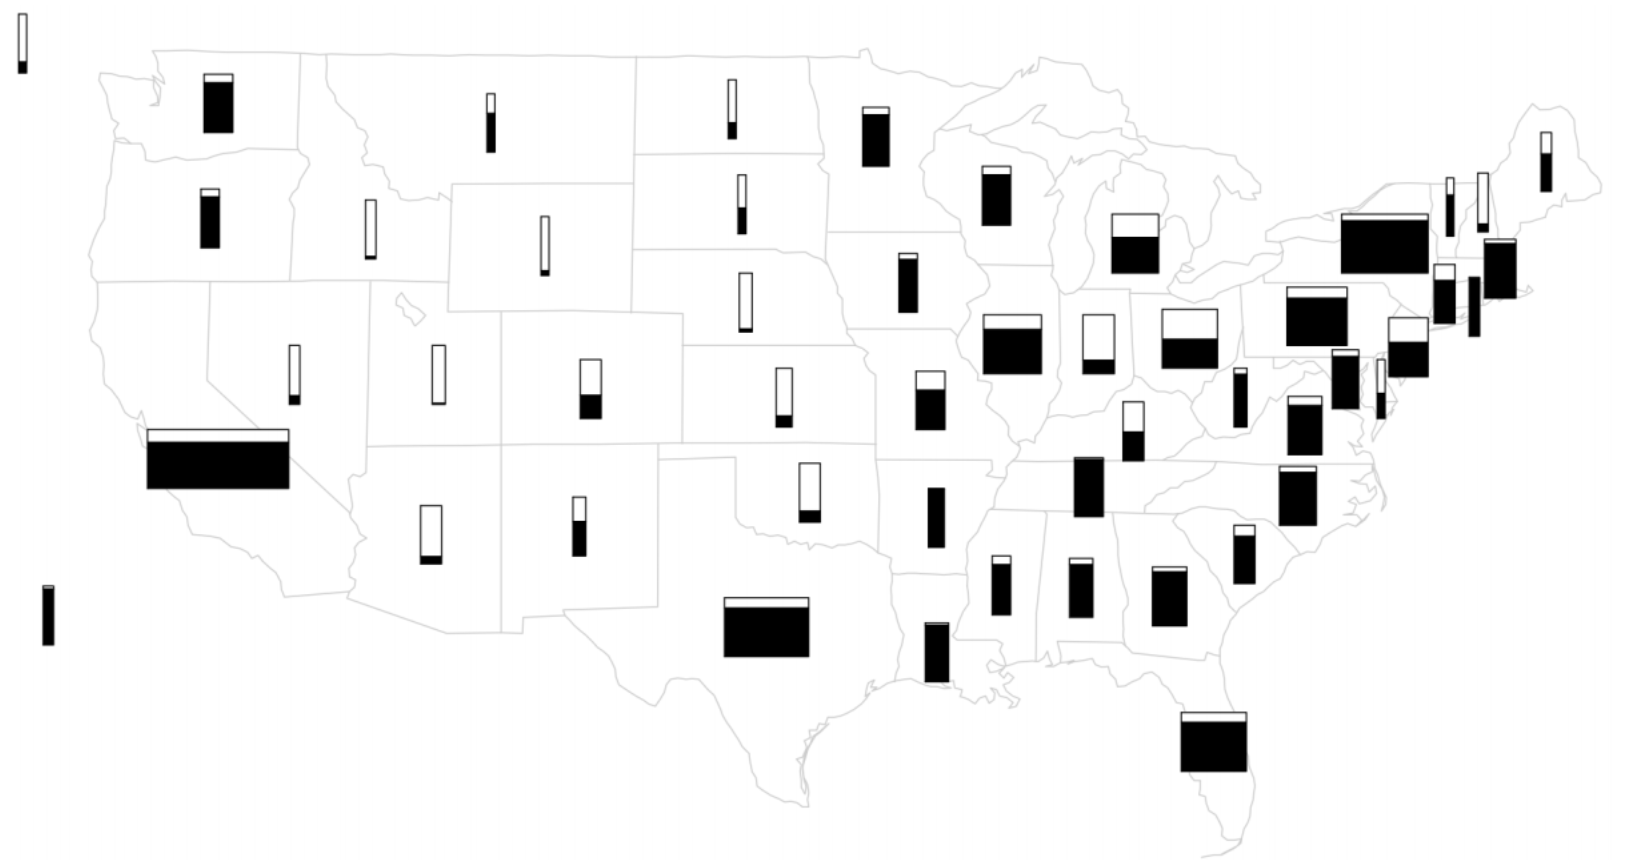
\includegraphics[width=0.8\textwidth]{election.png}
\end{center}
\caption{(BDA figure 6.1) Forecast of 1992 US presidential election. For each state, the height of the black bar indicates the probability of Clinton winning the election, and the width is the number of electoral votes. Polls from Texas and Florida not used in the forecast indicated much less support for Clinton than predicted, indicating a possible inadequacy of the model.}
\end{figure}




\section{Posterior predictive checking}

The basic idea of  posterior predictive model checking is that the observed data set should look ``typical'', relative to replicate data sets sampled from the posterior predictive distribution.

\subsection*{Example: Newcomb's speed of light measurements}
\begin{itemize}
\item Figure \ref{figure:newcomb} (top) shows  66 measurements of the speed of light made by Simon Newcomb in 1882. This is a classic example of a data set with outliers. Note that the lowest two measurements are significantly lower than the rest. (Incidentally, Newcomb threw out the lowest one, but kept the second lowest one.)
\item A naive approach would be to model the data as $\N(\mu,\sigma^2)$. In this case, we can visually see that there may be issues with this, but in more complicated, high-dimensional situations, it is usually difficult to visually assess whether a model will fit. Let's see what happens if we use the normal model.
\item Figure \ref{figure:newcomb} (bottom) shows 20 replicate data sets sampled from the posterior predictive (see BDA for prior details).  Each of these was generated by first sampling $(\mu,\sigma^2)$ from the posterior, and then sampling 66 points $x_i^\text{rep}$ from a normal with this mean and variance (i.e., using the same mean and variance for all 66).
\item Visually, none of these look much like the original observed data set. To quantify this, Figure \ref{figure:newcomb-min} shows a histogram of the 20 minimum values, $\min x_i^\text{rep}$, obtained from the 20 replicate data sets, compared to the observed minimum value, $\min x_i$. The minimum is just one possible choice of statistic that could be used to check the model fit.
\end{itemize}


\begin{figure}
\begin{center}
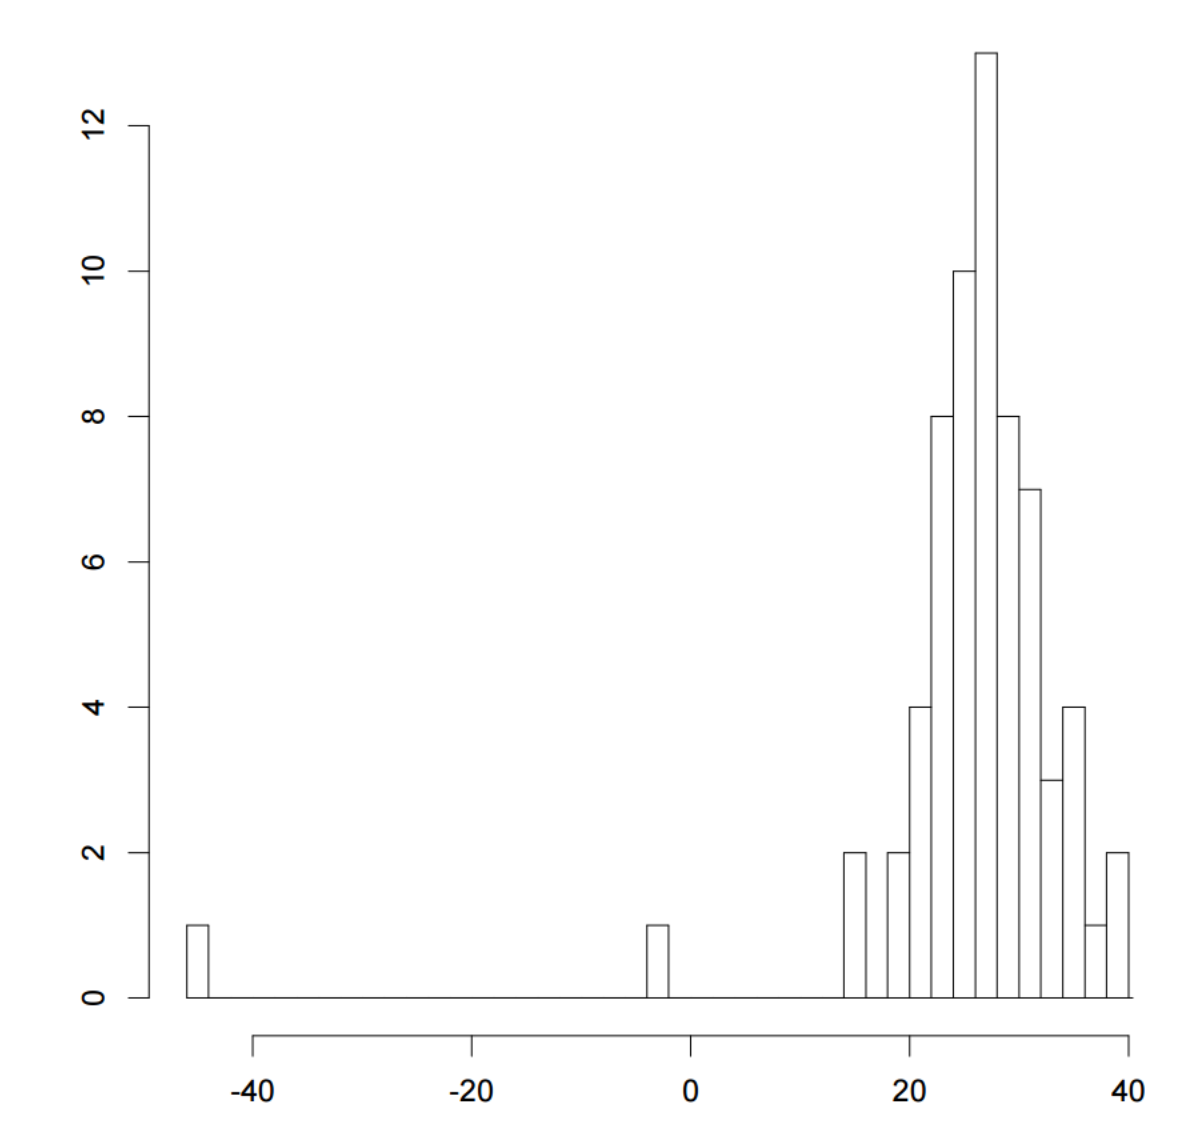
\includegraphics[width=0.6\textwidth]{newcomb.png}\\
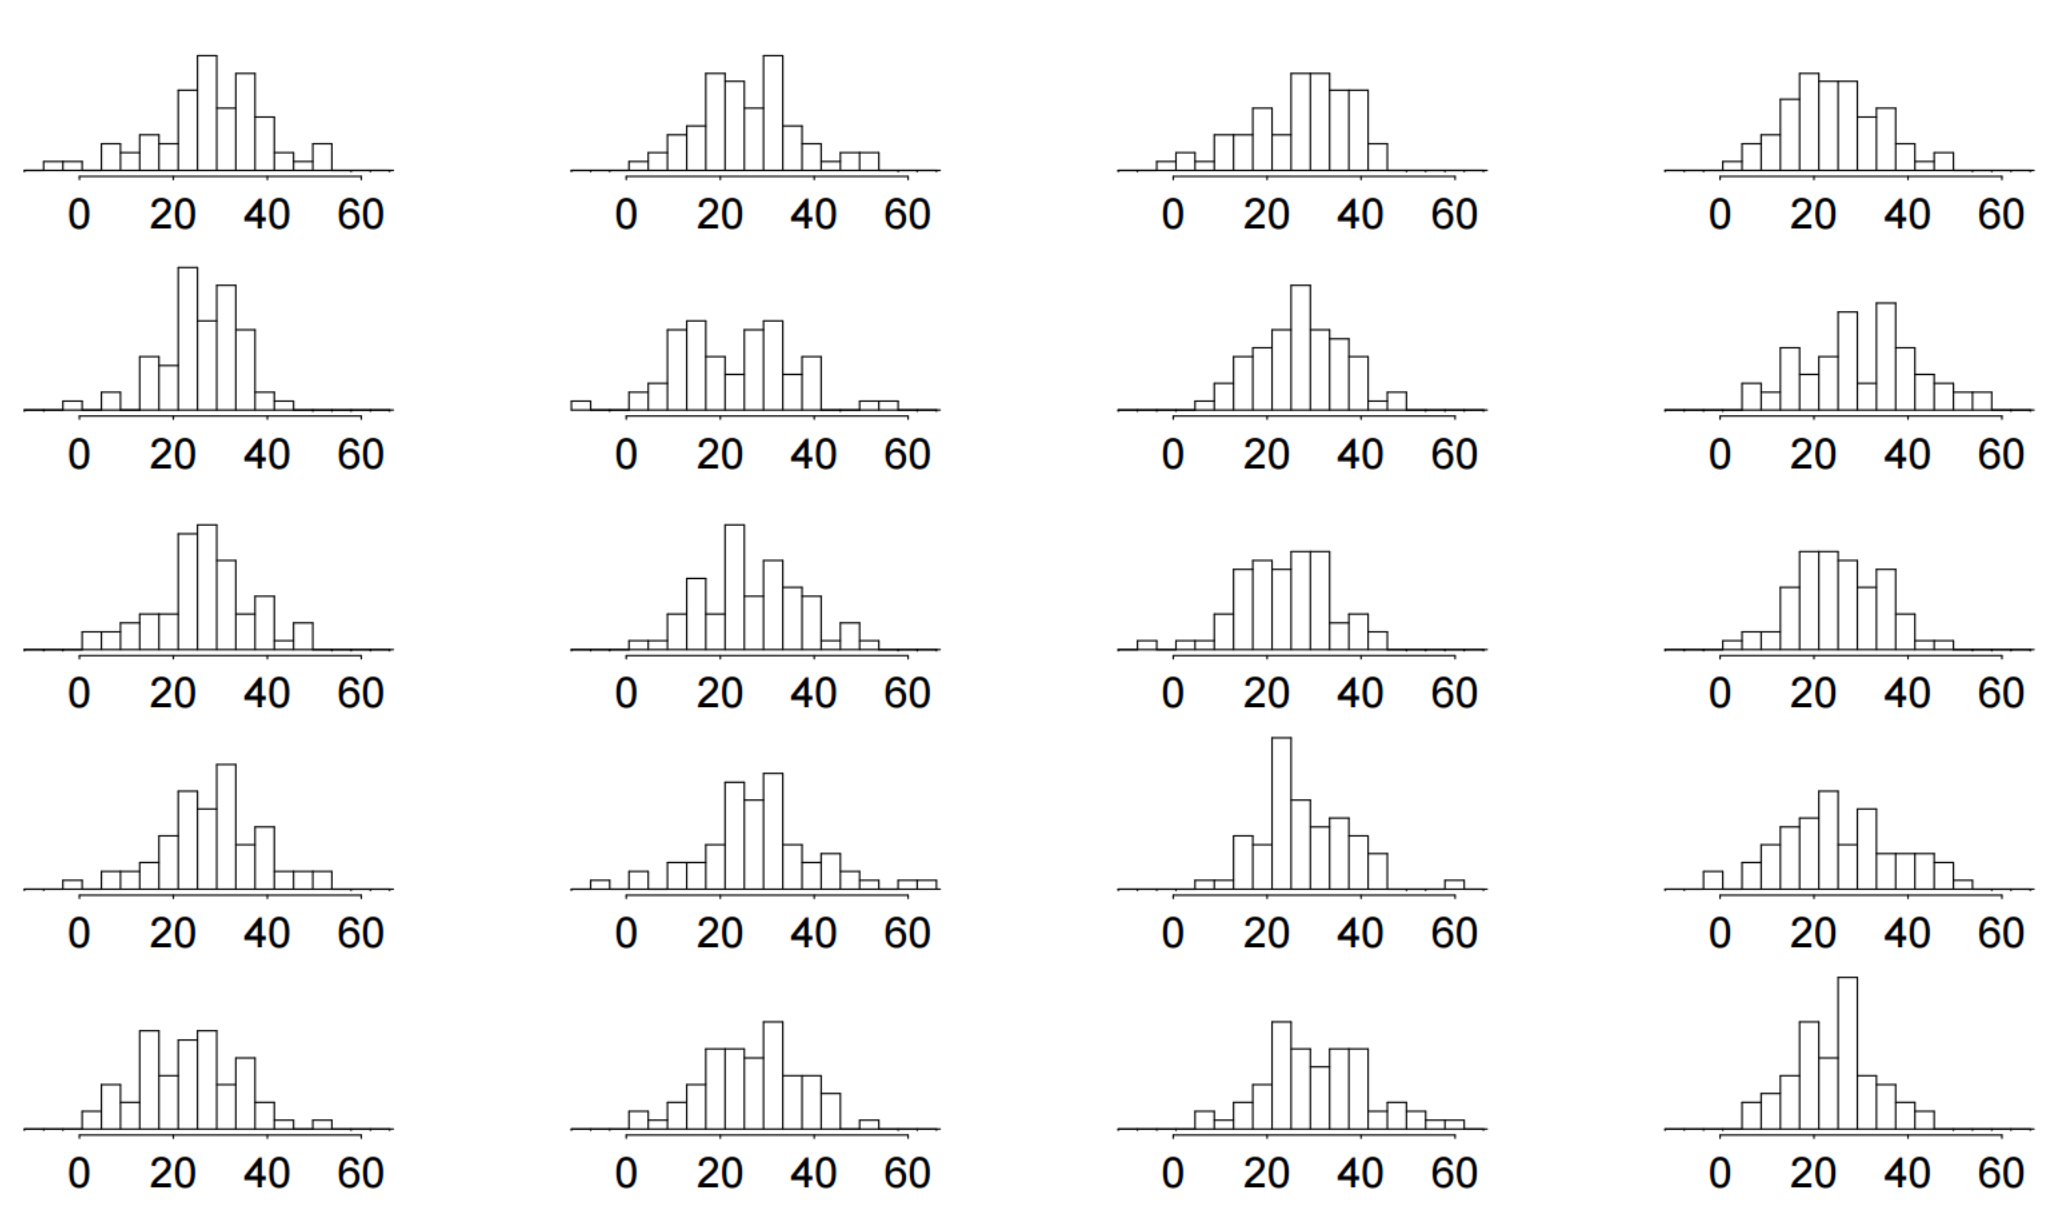
\includegraphics[width=1.0\textwidth]{newcomb-rep.png}
\end{center}
\caption{\\Top: (BDA figure 3.1) Histogram of 66 measurements of the speed of light made by Simon Newcomb (Stigler, 1977). (See BDA for details.)\\
Bottom: (BDA figure 6.2) Twenty replicate data sets from the posterior predictive distribution under a normal model, given the Newcomb data.}
\label{figure:newcomb}
\end{figure}


\begin{figure}
\begin{center}
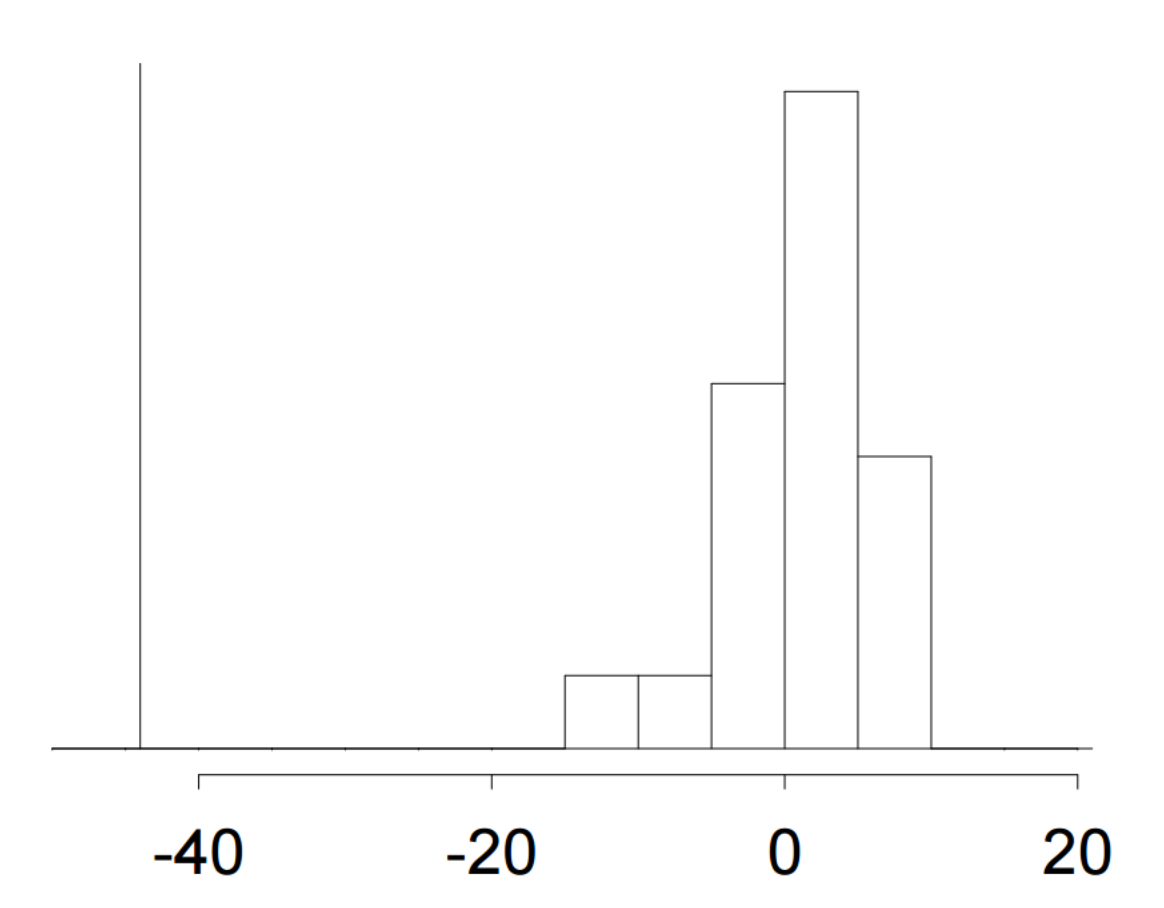
\includegraphics[width=0.5\textwidth]{newcomb-min.png}
\end{center}
\caption{(BDA figure 6.3) Histogram of the minimum values over the 20 replicate data sets, compared with the minimum value from the observed data set (the vertical line at around $-45$).}
\label{figure:newcomb-min}
\end{figure}


\subsection*{The idea of posterior predictive checks}
\begin{itemize}
\item If by some miracle the likelihood is exactly correct, and we have a very large amount of data, then the posterior should be highly concentrated at the true parameter value, and the distribution of the observed data should be basically identical to the distribution of the replicate data sets. However, this is more than we can hope for.
\item On the other hand, if the likelihood or prior are way off, then basically none of the replicate data sets will look like the observed data set. This is bad.
\item If the likelihood and prior are close enough to being correct, relative to the amount of data, then some of the replicate data sets should look roughly like the observed data set. This is what we aim for.
\item The nice thing about posterior predictive checks (as opposed to something like cross-validation) is that they are usually much less computationally intensive, since they only involve generation of replicate data sets (which is usually relatively easy), as opposed to computing the posterior for multiple data sets.
\end{itemize}



\subsection*{Definition of posterior predictive for replicate data sets}
\begin{itemize}
\item Recall that the posterior predictive distribution of a single future sample is 
$$p(x_{n +1}| x_{1:n}) = \int p(x_{n +1} | \theta)p(\theta | x_{1:n}) d \theta $$
(assuming the data is conditionally independent given $\theta$).
\item Here, we will be considering the posterior predictive distribution of an entire replicate data set, $x_{1:n}^\text{rep}$,
$$ p(x_{1:n}^\text{rep} | x_{1:n}) = \int p(x_{1:n}^\text{rep} | \theta)p(\theta | x_{1:n}) d \theta. $$
\item We can sample from the posterior predictive distribution on replicate data sets by first sampling $\theta | x_{1:n}$, and then sampling $x_{1:n}^\text{rep}| \theta$.  To sample $S$ replicate data sets, we would sample $\theta^1,\ldots,\theta^S$ i.i.d.\ $\sim p(\theta | x_{1:n})$, and then sample $x_{1:n}^{\text{rep,}s} | \theta^{s}$ for $s = 1,\ldots,S$.
\end{itemize}


\subsection*{Test statistics and test quantities}
\begin{itemize}
\item To perform a posterior predictive check, we compare the observed value of some test statistic/quantity to its distribution under the posterior predictive.
\item Test statistic = function of the data only, $T(x_{1:n})$.
\item Test quantity = function of data and parameter, $T(x_{1:n},\theta)$. This is a generalization that can be useful in the Bayesian context.
\item The speed of light example used the test statistic $T(x_{1:n}) = \min x_i$. 
\item Using different test statistics/quantities will allow you to probe different aspects of model fit.
\end{itemize}

\subsection*{Posterior predictive p-values}
\begin{itemize}
\item To simplify the notation, let's abbreviate $x = x_{1:n}$.
\item Recall that the classical frequentist p-value for a test statistic $T(x)$ is defined as
$$p_C = \Pr\big(T(X)\geq T(x) \mid \theta_0 \big),$$
where $x$ is the observed data, $X$ is distributed according to $P_{\theta_0}$, and $\theta_0$ usually corresponds to the null hypothesis. The idea is that if the p-value is very small, then the observed data is very atypical under the null hypothesis, providing evidence for rejecting the null.
\item The posterior predictive p-value for $T(x)$ is defined as
$$p_B = \Pr\big(T(X^\rep)\geq T(x) \mid x \big),$$
or more generally, for a test quantity $T(x,\theta)$,
$$p_B = \Pr\big(T(X^\rep,\theta)\geq T(x,\theta) \mid x \big).$$
In this expression, $x$ is fixed and equal to the observed data, and $(X^\rep,\theta) | x$ is distributed according to 
$$p(x^\rep,\theta | x) = p(x^\rep | \theta) p(\theta | x), $$
which can be sampled from according to the same process as described above.
\item Using such samples, we can make a Monte Carlo approximation,
$$ p_B \approx \frac{1}{S}\sum_{s = 1}^S \1 \big(T(x^{\rep,s},\theta^s)\geq T(x,\theta^s) \big). $$
\end{itemize}

\begin{figure}
\begin{center}
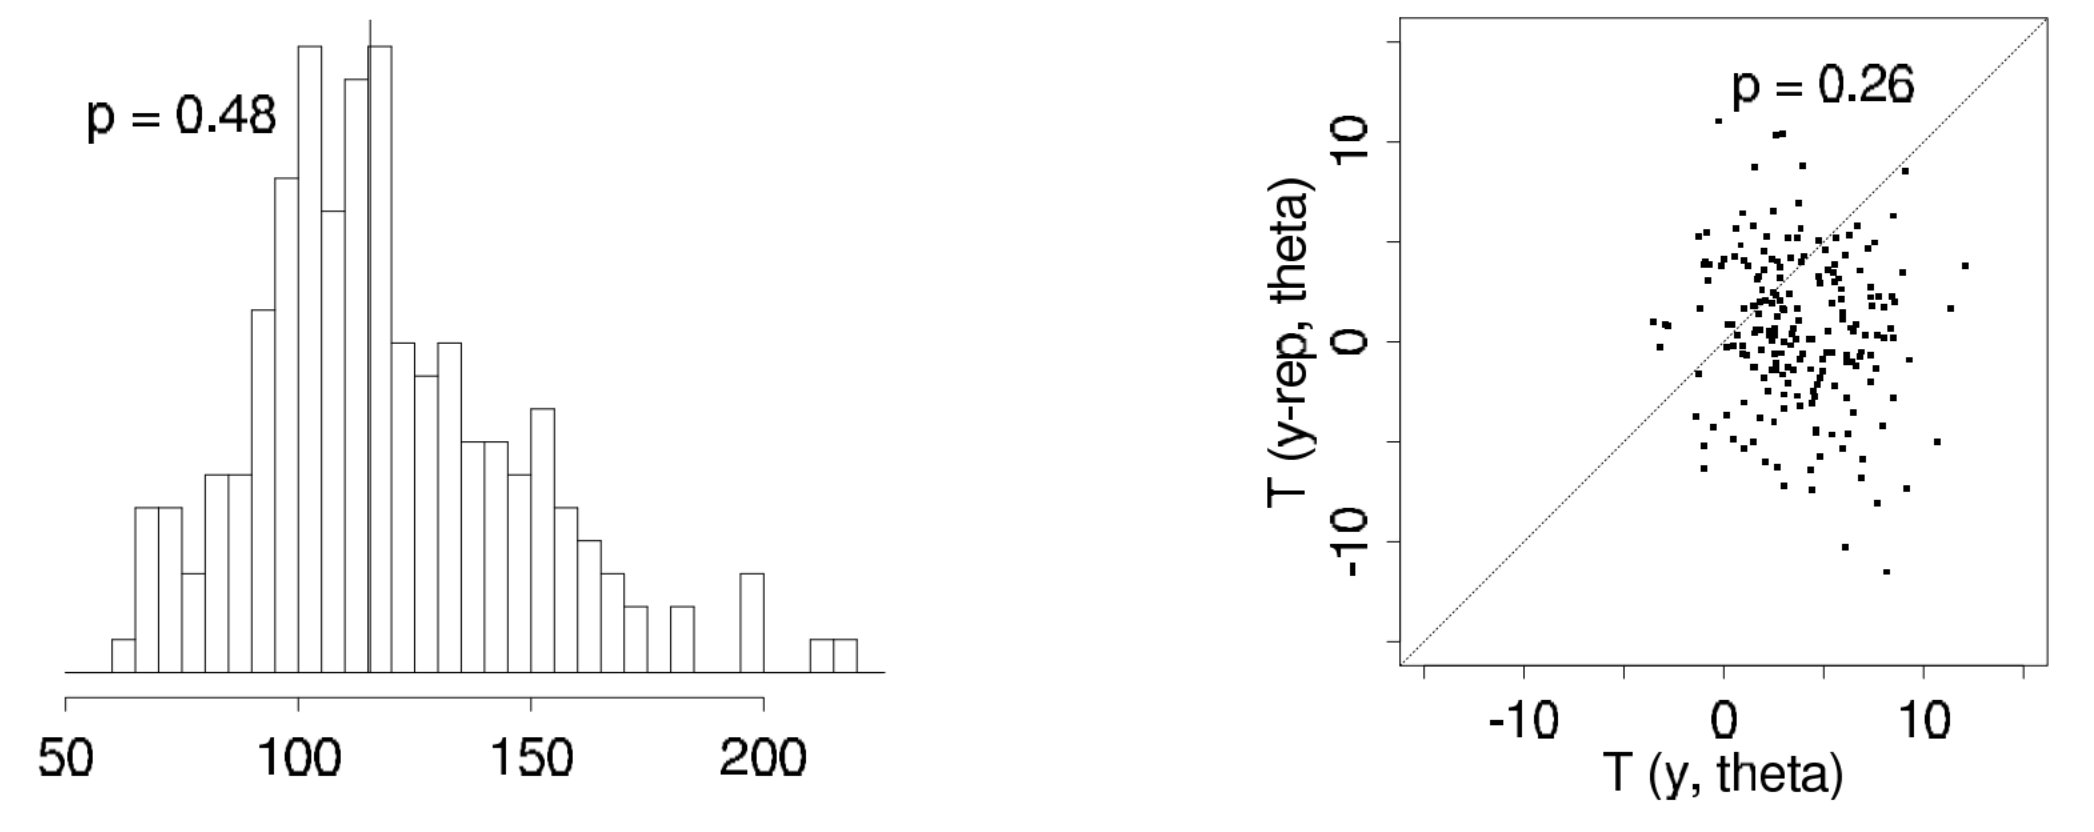
\includegraphics[width=1.0\textwidth]{newcomb-more.png}
\end{center}
\caption{(BDA figure 6.4) Left: Histogram of the sample variance over the 200 replicate data sets, compared with the observed sample variance. Right: Scatterplot of $T(x,\theta)$ versus $T(x^\rep,\theta)$ for the asymmetry statistic; the p-value is the fraction of points above the diagonal.}
\label{figure:newcomb-more}
\end{figure}

\subsection*{Example: Speed of light (continued)}
\begin{itemize}
\item How well is the model capturing the variance? Choose $T(x) = \hat \sigma^2$. The p-value is around 0.48, indicating that the model is doing okay (see figure \ref{figure:newcomb-more}).  However, the sample variance is a poor choice of test statistic for this model, since it is a sufficient statistic, so the model is already paying very close attention to matching it. Consequently, it isn't really helping us recognize poor model fit.
\item How well is the model capturing any asymmetry of the distribution? We can compare distance from the 90\% and 10\% quantiles to the center, $\theta$:
$$ T(x,\theta) = | x_{(61)} - \theta | - | x_{(6)} - \theta |. $$
Here, $x_{(j)}$ indicates the $j$th order statistic.  The p-value is around 0.26, so the model seems to be doing okay in this respect as well.
\end{itemize}

\subsection*{Interpretation of posterior predictive checks}
\begin{itemize}
\item The primary purpose of posterior predictive checks is not to construct hypothesis tests, but rather, to explore and visualize how well the model is capturing various aspects of the data distribution.
\item Consequently, it is not really that important whether you compute the p-value using an upper tailed (as above), lower tailed, or two-tailed approach---whenever the p-value is very close to zero or one, this is a flag that something may be amiss.
\item As usual, if you are computing multiple p-values, it is important to be aware of the fact that some of them may be small or large simply by chance---i.e., remember the multiple testing issue. Since we are not constructing a formal hypothesis test, however, it is sufficient to just keep this in mind when interpreting the results.
\item Ideally, a frequentist p-value is uniformly distributed over the interval from 0 to 1. Posterior predictive p-values do not always have this property, which can complicate their interpretation somewhat. This is another reason to view them as tools for exploratory purposes, rather than precisely calibrated tests of model fit.
\item It's also important to remember that each posterior predictive check is only assessing model fit with respect to one particular statistic. So, even though things might look okay for a given statistic, there might be issues with other aspects of the distribution you haven't considered.
\item What should you do if your posterior predictive check indicates a problem? In some cases, the inferences you draw from the model might not be negatively affected by the lack of model fit---if you are certain of this, then it might still be okay to use the model. Otherwise, the results of the posterior predictive check can provide valuable insight into how to modify the model in order to improve it. 
\item If you do modify the model, however, it is crucial to ensure that you do not overfit---after all, you could match every statistic perfectly by using a model which simply reproduces the observed data set every time!
\end{itemize}


\section{Example: random effects model of adolescent smoking}

\subsection*{Data/setup}
\begin{itemize}
\item (This is the example starting on page 148 of the BDA.)
\item 2000 Australian adolescents (teenagers)
\item Smoking behavior was recorded every six months, for three years. (Figure \ref{figure:smoking})
\item Questions of interest: How well can smoking behavior be predicted based on parental smoking and other background variables? At what ages do boys and girls start smoking?
\end{itemize}

\begin{figure}
\begin{center}
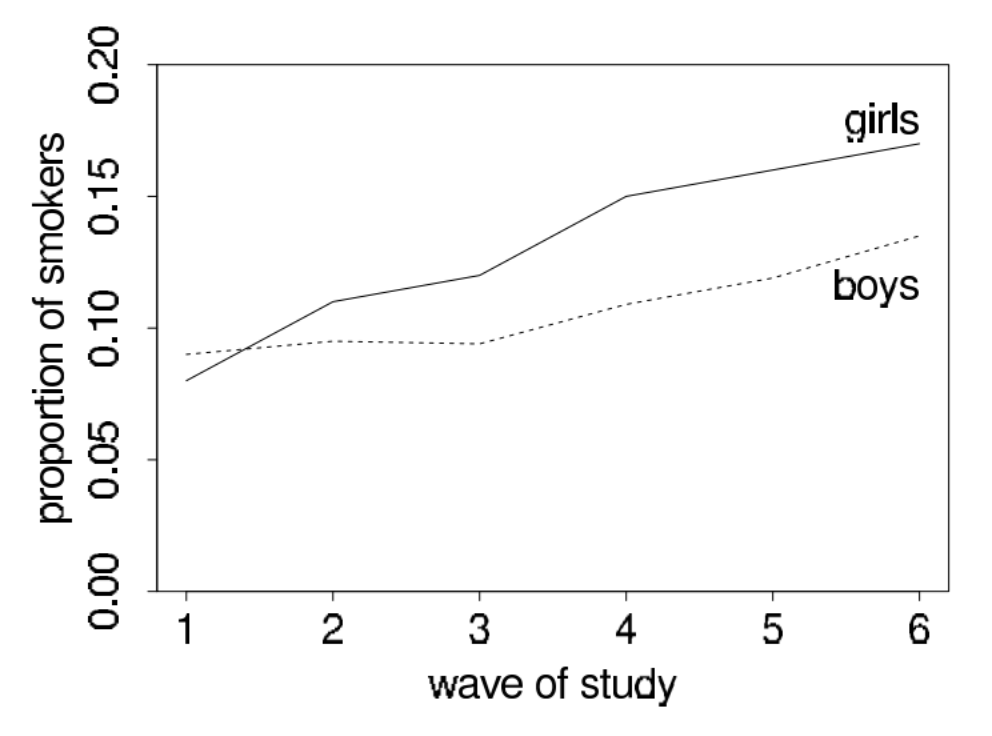
\includegraphics[width=0.7\textwidth]{smoking.png}
\end{center}
\caption{(BDA figure 6.6) Fraction of boys and girls in the study who were smoking at each time (wave) $t = 1,\ldots,6$.}
\label{figure:smoking}
\end{figure}

\subsection*{Model 1: Logistic regression with random effects}
\begin{itemize}
\item Covariates used: 
\begin{itemize}
\item[] $x_{j 1} = \1(\text{parent smokes})$
\item[] $x_{j 2} = \1(\text{female})$
\end{itemize}
\item Target variables: For each person $j$, for times $t= 1,\ldots,6$,
\begin{itemize}
\item[] $y_{j t} = \1(\text{person $j$ is smoking at time $t$})$
\end{itemize}
\item Target variables are modeled as:
$$ Y_{j t}| x,\beta,\alpha\sim \Bernoulli\Big(\logit^{-1}\big(\beta_0+ \beta_1 x_{j 1} + \beta_2 x_{j 2} + \beta_3(1 - x_{j 2}) t + \beta_4 x_{j 2} t + \alpha_j\big)\Big)$$
\item $\logit(p) = \log (p/(1 - p))$ and $\logit^{-1}(a) = e^a/(1+e^a)$
\item $\alpha_j$ is referred to as a ``random effect'' or ``individual effect'' for person $j$. (The term ``random effect'' is misleading, but unfortunately common--- in this case, it just means that there is a different value for each person.)
\item Priors: $\alpha_j \sim \N( 0,\tau^2)$, improper uniform priors on $\beta,\tau$. (Incidentally, it's generally a bad idea to assume a parametric prior for the individual effects $\alpha_j$, since the number of parameters is growing with the size of the data set, and this can lead to lack of consistency if this prior is even slightly wrong. This can be fixed by using an inference method which eliminates the individual effects in some way or by placing a nonparametric prior on them.)
\end{itemize}

\subsection*{Model 2: Mixture of model 1 and a zero component}
\begin{itemize}
\item Assume each person $j$ has an unobserved ``susceptibility'' $S_j$, which is 1 if the person might possibly smoke, and 0 if she/he will never smoke no matter what.
\item These are modeled as
$$  S_j|\gamma \sim \Bernoulli\big(\logit^{-1}(\gamma_0+ \gamma_1 x_{j 1} + \gamma_2 x_{j 2}) \big) $$
\item Given $S_j = 1$, $Y_j$ is distributed as in model 1, and given $S_j = 0$, $Y_j = 0$ with probability 1.
\item Improper uniform priors on $\gamma$'s. 
\end{itemize}

\subsection*{Posterior predictive checks of the two models}
\begin{itemize}
\item Test statistics:
\begin{itemize}
\item fraction of subjects who never smoked during the study
\item fraction of subjects who always smoked during the study
\item fraction of subjects who started smoking during the study and did not stop smoking (``incident smokers'')
\end{itemize}
\item Results:
\begin{center}
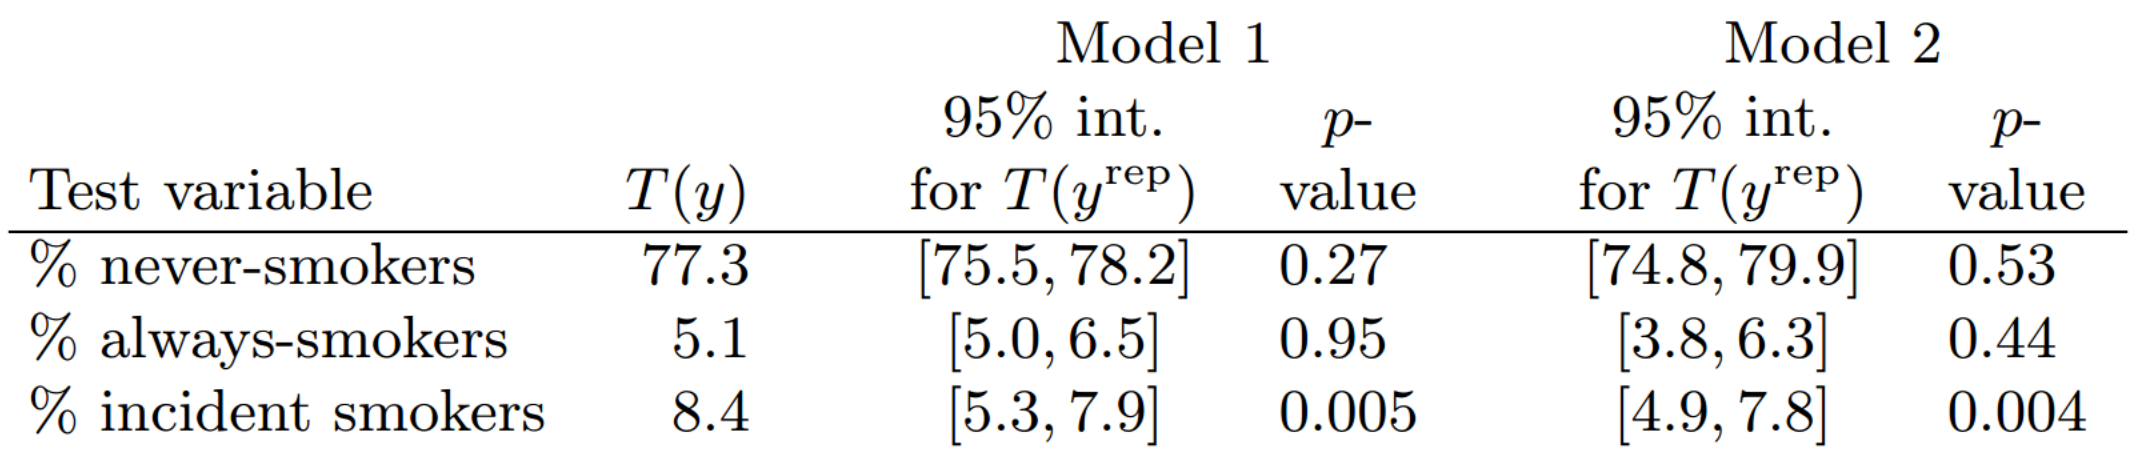
\includegraphics[width=1\textwidth]{smoking-results.png}
\end{center}
\item Both models capture the fraction of never-smokers well.
\item Model 2 captures the fraction of always-smokers much better than model 1.
\item Neither model captures the fraction of incident smokers very well. (P-values this small will only occur by chance about 1 in 200 times, and we have only looked at three p-values.)
%\item Note: The purpose here is not to use this as a criterion for selecting one of these models. The purpose of comparing the two models is simply to illustrate how the results may vary for different models.
\end{itemize}


\section{Related methods}

\subsection{Graphical checks}
\begin{itemize}
\item Rather than looking at a single test statistic $T(x)$, sometimes it is useful to look at a bunch of test statistics $T_1(x),\ldots,T_d(x)$ simultaneously.
\item BDA refers to this as a graphical posterior predictive check, since the model fit is assessed by visual inspection of some graphical display of $(T_1(x),\ldots,T_d(x))$.
\item In this case, rather than displaying the posterior predictive distribution of the test statistics/quantities in a histogram, you would typically display one or several samples of the test quantities.
\item Example: See Figure \ref{figure:graphical}. See BDA section 6.4 for details.
\end{itemize}

\begin{figure}
\begin{center}
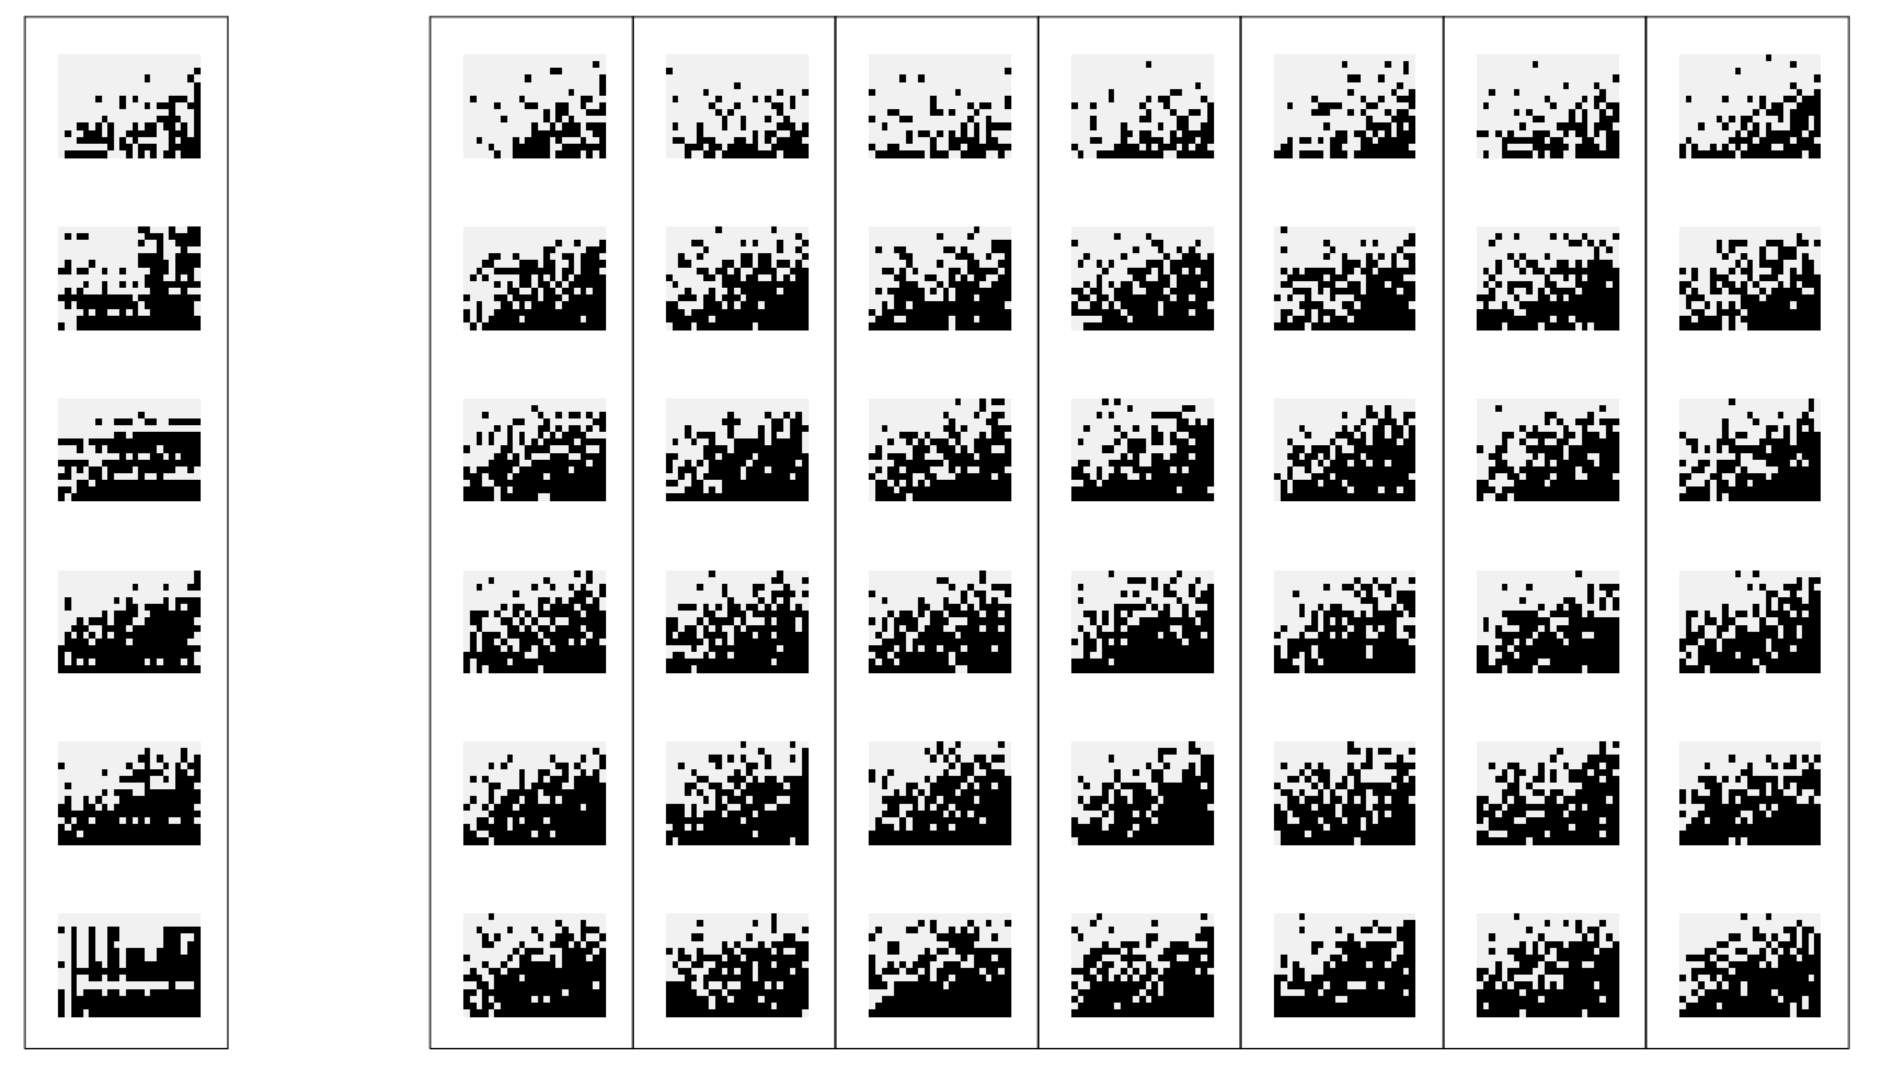
\includegraphics[width=1\textwidth]{graphical.png}
\end{center}
\caption{(BDA figure 6.7) Left: Observed data is a binary matrix of responses for each of 6 subjects. Right: Seven samples from the posterior predictive distribution for the 6 subjects.}
\label{figure:graphical}
\end{figure}



\subsection{Comparing posterior samples to the prior}

\subsubsection*{The basic idea}
\begin{itemize}
\item If the model were perfect (i.e., both the likelihood and the prior were correct), then for a typical data set $x$, a sample from the posterior should look like a sample from the prior. Note: The claim here is not that $p(\theta | x)$ will look like $p(\theta)$, but rather that if we were to draw $\theta_0\sim p(\theta)$, draw $x_0\sim p(x|\theta_0)$ (so that $x_0$ is a ``typical'' data set under the model), and then draw $\theta_1\sim p(\theta|x_0)$, then $\theta_1$ is actually distributed according to the prior, $p(\theta)$.
\item For this reason, it can be useful to compare posterior samples to the prior, particularly in models with a large number of parameters.
\end{itemize}

\begin{figure}
\begin{center}
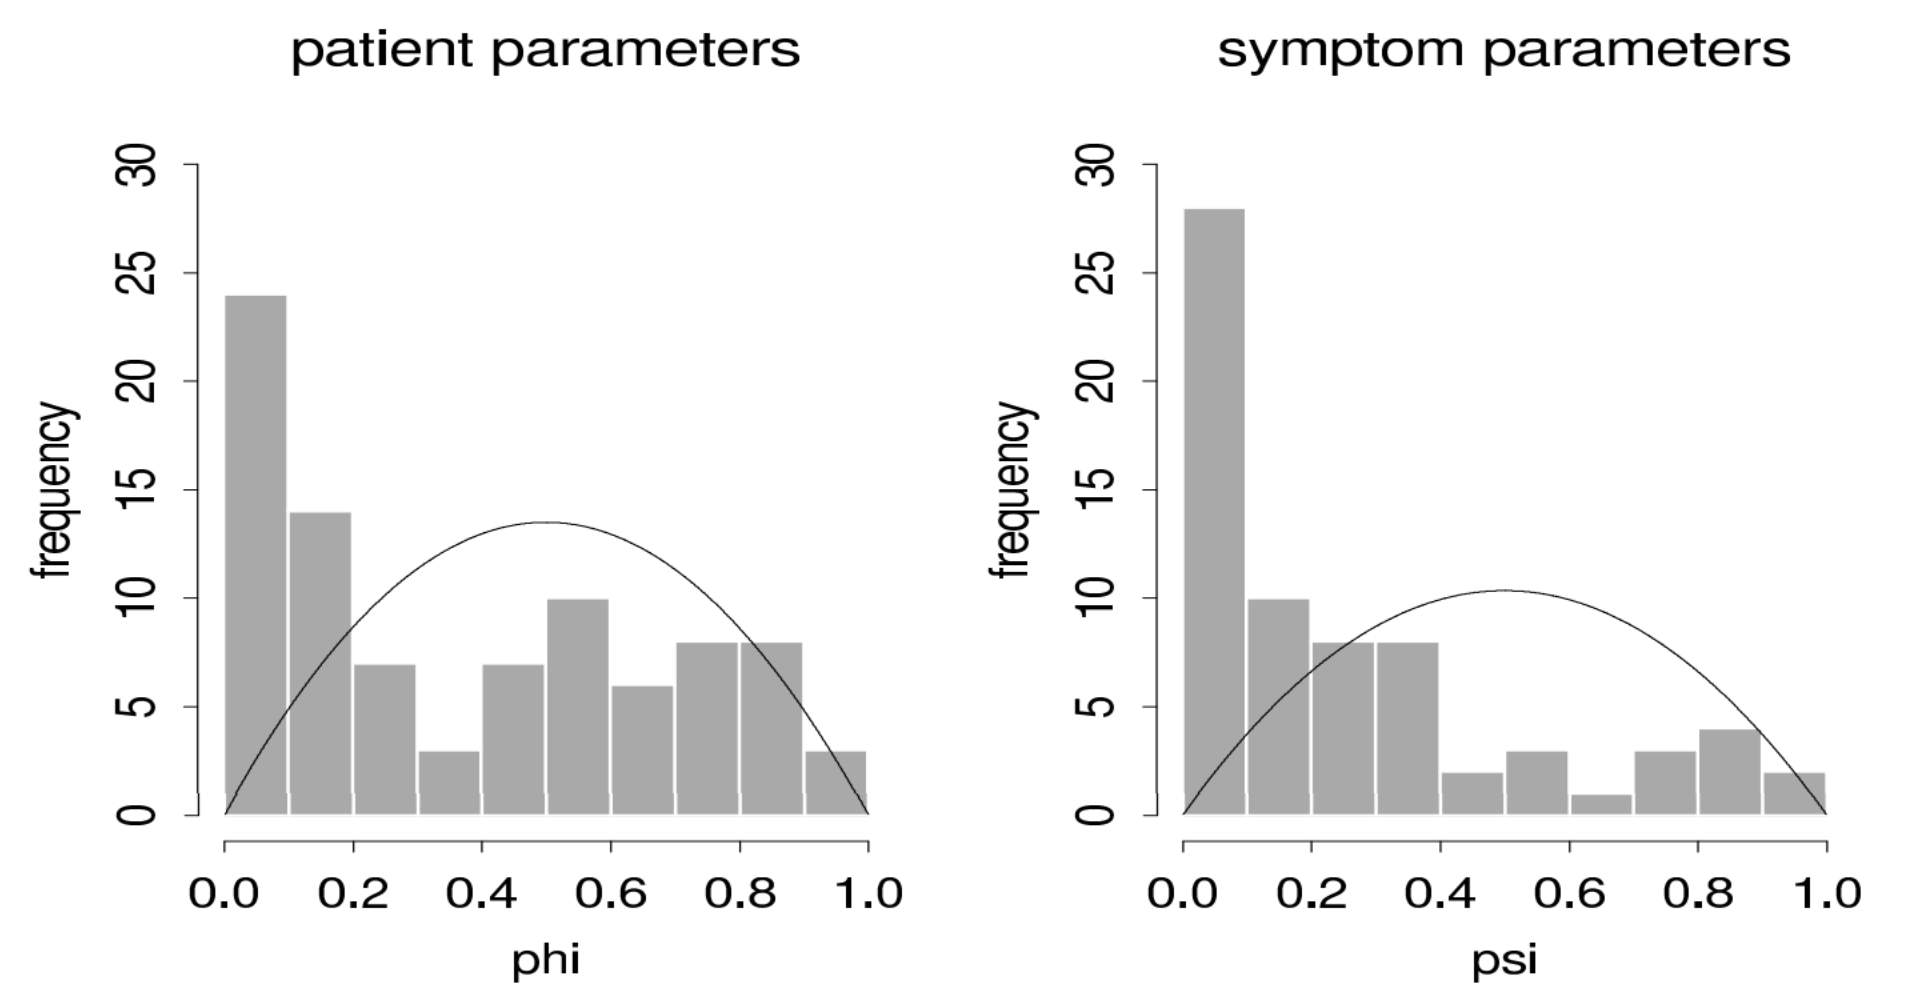
\includegraphics[width=0.7\textwidth]{psychology-1.png}
\end{center}
\caption{(BDA figure 6.9) Left: Histogram of $\phi_1,\ldots,\phi_{90}$, for a single sample from the posterior, compared with the density of the prior, $\Beta(2,2)$. Right: Same for $\psi_1,\ldots,\psi_{69}$.}
\label{figure:psychology-1}
\end{figure}

\begin{figure}
\begin{center}
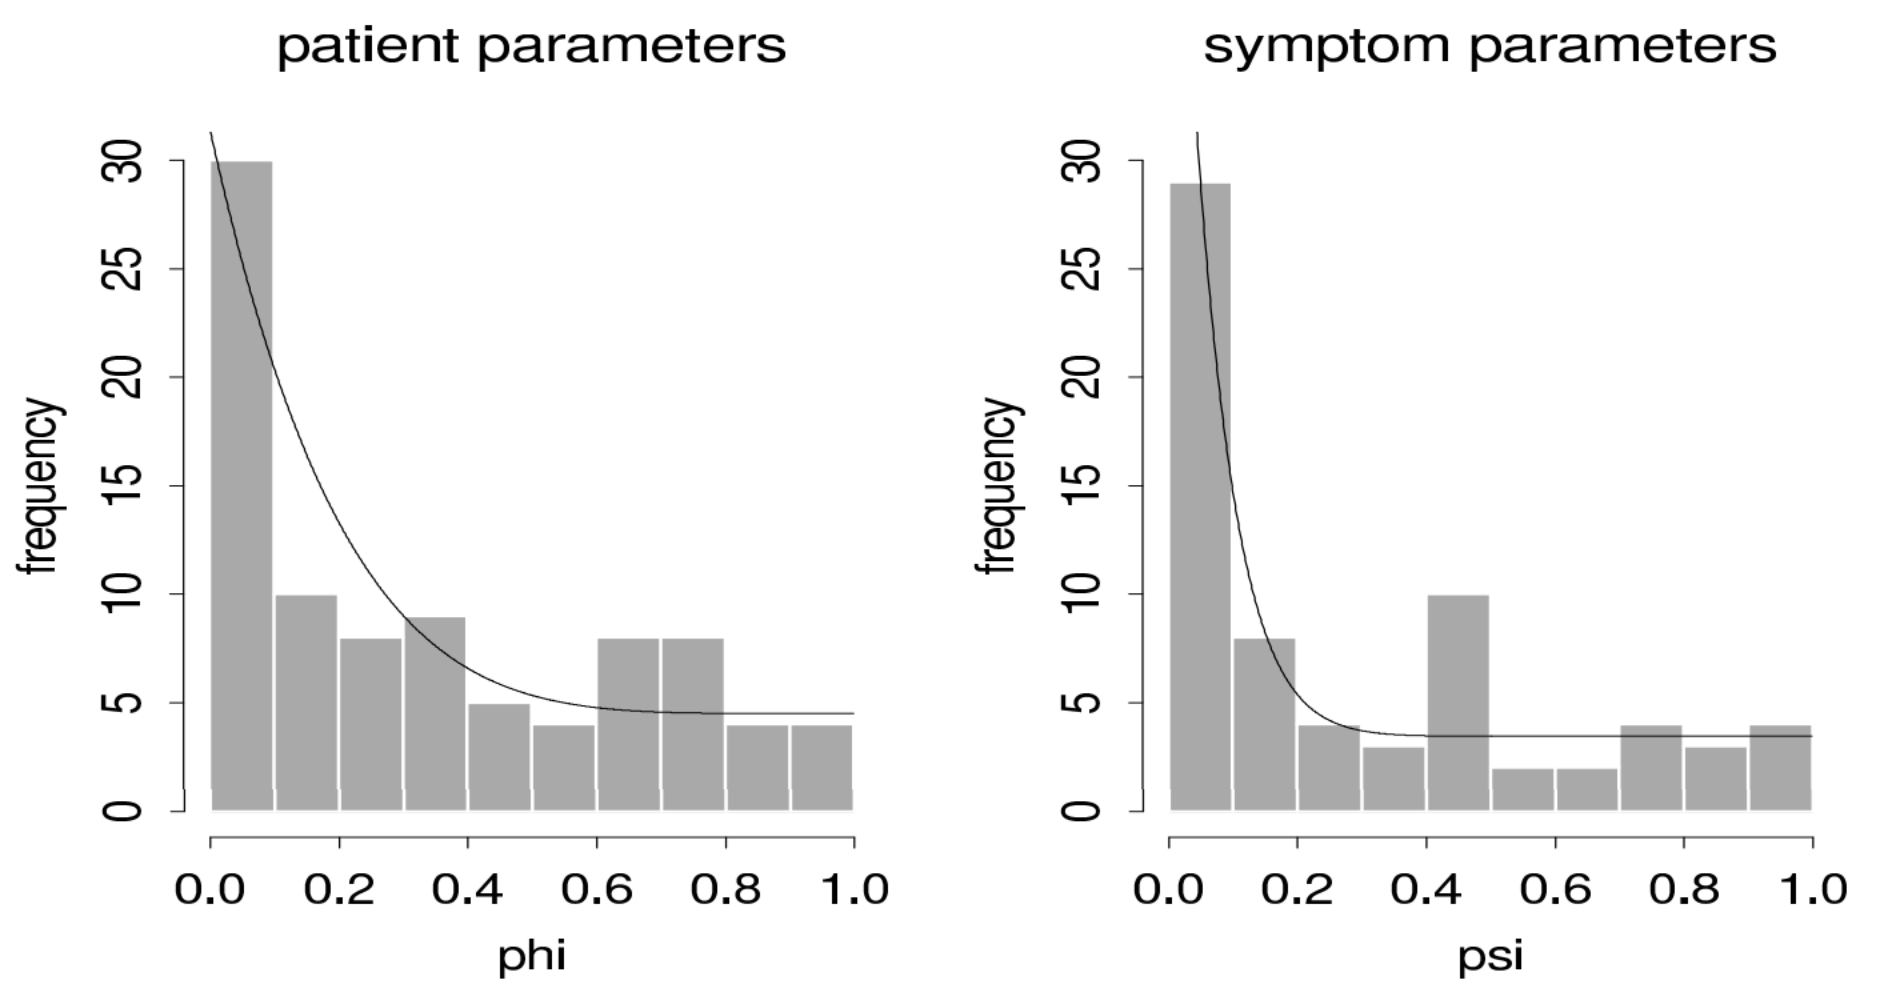
\includegraphics[width=0.7\textwidth]{psychology-2.png}
\end{center}
\caption{(BDA figure 6.10) Same as Figure \ref{figure:psychology-1}, with the revised prior.}
\label{figure:psychology-2}
\end{figure}


\subsubsection*{Example}
\begin{itemize}
\item (This is the example on page 155 of BDA.)
\item It just so happens that in this example, the test quantities are functions of $\theta$ only (and not $x$), but that is just a coincidence.
\item This example involves a hierarchical model from psychology (the details are not important) that has parameters $\phi_1,\ldots,\phi_{90}$ and $\psi_1,\ldots,\psi_{69}$ corresponding to patients and psychological symptoms.
\item Independent $\Beta(2,2)$ priors were placed on all of these parameters. If the model (including prior) were correct, then for a typical data set, these parameters should look roughly like draws from a $\Beta(2,2)$ distribution.
\item However, Figure \ref{figure:psychology-1} indicates that this is not the case.
\item The prior was revised to use mixtures of beta distributions:
\begin{align*}
\phi_j & \sim \tfrac{1}{2} \Beta(1,6) + \tfrac{1}{2}\Beta(1,1)\\
\psi_j & \sim \tfrac{1}{2} \Beta(1,16) + \tfrac{1}{2}\Beta(1,1).
\end{align*}
\item Figure \ref{figure:psychology-2} indicates that the posterior sample is more concordant with the prior, when using this revised prior.
\end{itemize}



\section{Cross-validation}

\subsection*{The basic idea}
\begin{itemize}
\item Often, the ideal way of evaluating a statistical method is to see how well it generalizes to new data.
\item We could simulate such an evaluation by splitting the observed data set into a ``training'' set $T$ and a ``held-out'' set $H$, running the method on $T$ as if it were all of the observed data, and then evaluating its performance $H$ as if this were new data.
\item The basic idea of cross-validation is to do this for multiple splits $(T_1,H_1),\ldots,(T_k,H_k)$, and average the results.
\item Cross-validation is most often used for assessing predictive models of $y|x$ (such as in regression or classification problems), but it can also be used when modeling the distribution of $x$ alone.
\item Cross-validation is probably the most commonly-used method of choosing among competing models. It can also be used to estimate the generalization performance of a single model of interest.
\item The great thing about cross-validation, compared to many other model selection criteria, is that it is directly getting at what matters---how well does the method generalize. The crappy thing is that it requires you to run your method on multiple training sets, which takes time.
\end{itemize}

\subsection*{Common schemes}
\subsubsection*{Leave-one-out cross-validation (LOO-CV)}
\begin{itemize}
\item Involves $n$ splits: $(T_i,H_i)$ for $i = 1,\ldots,n$.
\item $H_i = \{i \}$ (i.e., data point $i$ only).
\item $T_i = \{1,\ldots,n \} \setminus H_i$ (i.e., everything else).
\end{itemize}

\subsubsection*{$k$-fold cross-validation}
\begin{itemize}
\item Involves $k$ splits: $(T_i,H_i)$ for $i = 1,\ldots,k$.
\item Divide the data set into $k$ disjoint (i.e., non-overlapping) subsets $S_1,\ldots,S_k$ that are equally sized, or roughly equally sized. 
\item $H_i = S_i$ and $T_i = \bigcup_{j\neq i} S_j$.
\item Note that LOO-CV is a special case of $k$-fold CV in which $k = n$.
\end{itemize}

\subsubsection*{Choosing $k$}
\begin{itemize}
\item LOO-CV: Low bias (good), high variance (bad). More computation (bad) --- except in special cases where tricks are possible.
\item 2-fold CV: High bias (bad), low variance (good). Less computation (good).
\item $k$-fold CV for well-chosen $k$: Juuust right.
\item It is standard to use $k = 10$ or maybe $k = 5$.
\end{itemize}


\subsection*{Measuring generalization performance}
\begin{itemize}
\item Suppose that when we run the method on training data $x_T = (x_i : i \in T)$, the generalization performance on a new data point $x$ is measured by a loss $\ell(x | x_T)$. 
\item Suppose we want to minimize the expected loss:
$$ \E_{p_0} \ell(X | x_T) = \int \ell(x | x_T)p_0(x) d x $$
where $p_0$ is the true distribution of the data. 
\item Examples:
\begin{itemize}
\item Log posterior predictive density / KL divergence. If we choose $$\ell(x | x_T) = - \log p(x | x_T),$$ where $p(x | x_T)$ is the posterior predictive density, then the expected loss is
$$ \E_{p_0} \ell(X | x_T) = -\int p_0(x) \log p(x | x_T) d x
 = D\big(p_0(x) \| p(x | x_T) \big) - H(p_0) $$
where $H(p_0) = -\int p_0 \log p_0$ is the entropy of $p_0$. So, basically, by choosing a model that minimizes this expected loss, we are trying to minimize the KL divergence from the true distribution.
\item 0-1 loss / probability of misclassification. In the classification setting, instead of just $x$'s, we have pairs $(x,y)$.  If we choose $$\ell(x,y | x_T,y_T) = \1(y \neq f_T(x)),$$ where $f_T(x)$ is the predicted value of $y$ corresponding to $x$ when the training set is $(x_T,y_T)$, then the expected loss is
$$ \E_{p_0} \ell(X,Y | x_T,y_T) = \int \1(y \neq f_T(x)) p_0(x,y) d x d y = \Pr(Y \neq f_T(X)),$$
which is the probability of misclassification.
\end{itemize}
\end{itemize}

\subsection*{A derivation of cross-validation}
\begin{itemize}
\item Suppose we would like to estimate $\E_{p_0} \ell(X | x_{1:n})$. At first, it might seem like a natural idea to form a Monte Carlo approximation of this expectation, using the observed data to approximate $p_0$: i.e. to use $\frac{1}{n} \sum_{j = 1}^n \ell(x_j | x_{1:n})$. However, if you think about it, this will tend to make the performance look better than it actually is, since it is evaluating performance on the same data that was used for training/estimation/inference.
\item If $T$ is a training subset, then
 $$ \E_{p_0} \ell(X | x_{1:n}) = \E_{p_0} \ell(X | x_T) + \text{bias}. $$
\item The bias will be larger when $T$ is small relative to $n$. There are methods for estimating the bias (see BDA page 175). However, if the only goal is to choose among competing models, this bias is often ignored (I guess the hope that the bias doesn't change too much from model to model).
\item Now, we can use a held-out set $H$ (disjoint from $T$) to form the Monte Carlo approximation
 $$\E_{p_0} \ell(X | x_T) \approx \frac{1}{| H |}\sum_{j \in H} \ell(x_j | x_T)$$
 without the issue of ``using the data twice.''
\item The cross-validation estimate of generalization performance is obtained by averaging these Monte Carlo approximations over all splits into training/held-out sets:
 $$\frac{1}{k} \sum_{i = 1}^k \frac{1}{| H_i |}\sum_{j \in H_i} \ell(x_j | x_{T_i}).$$
\end{itemize}



\end{document}

























